% ============================================================
% RESULTS -- report only, no interpretation.
% Written 2026-11-06 from results/analysis/FINAL_NOTES.md; review revision 2026-11-06 (per-pair effects first).
% 2026-11-08 ARS REVISION (notes/ARS_review_20261108/revision_roadmap.md; REV-01 and others): each subsection now
% opens with the plain finding and cites the tables instead of restating them. Detail that the main text restated
% (prompt-level GEE terms, scale disagreements, KL-cap binding counts, ARA export caveats, H3 decomposition,
% dev-set, re-score and search-convergence paragraphs) moved VERBATIM, with its src comments, to Appendix
% app:moved-results (sections/08i_revision_details.tex); five secondary figures (fig:gmpoa-dev, fig:seed-dev,
% fig:dev-generation, fig:kl-budget, fig:search-convergence) moved there too, labels unchanged. No existing number was
% changed. New numbers come from the revision_* scripts and CSVs (src comments name the file):
%   scripts/analysis/revision_seed_variance.py   -> results/analysis/revision_{sigma_*,heterogeneity,pair_variances}.csv
%   scripts/analysis/revision_kl_budgets.py      -> results/analysis/revision_kl_budget_*.csv
%   scripts/analysis/revision_h2_sensitivity.py  -> results/analysis/revision_h2_sensitivity*.csv
%   scripts/analysis/revision_outcome_classes.py -> results/analysis/revision_outcome_classes.csv
%   scripts/analysis/revision_misc_estimands.py  -> results/analysis/revision_{retention,kw_gap_abs,olmo_q3g}.csv
% "family" -> "pair" / "release pair" in the headline claims (REV-25); "error" -> "disagreement" (REV-33).
% Previous version: sections/05_results.tex.bak-20261108-rev.
% ============================================================
\section{Results}
\label{sec:results}

The study asked whether refusal removal is harder in the newer model of each
release pair (H1), whether this depends on the class of edit (H2), and whether
keyword counts agree with an automatic judge (H3). Outcomes are WildGuard
refusal rates on the 972 harmful held-out prompts for the selected seed-1
models; pp denotes percentage points. The release pair is the unit, so
per-pair effects with intervals that add run-to-run variance are the primary
evidence; prompt-level tests describe prompt sampling within a pair
(\S\ref{sec:setup-stats}). Detail that earlier drafts gave here is in
Appendix~\ref{app:moved-results}.
% src: results/analysis/h1h2_tests.csv (n_in_family 23 / 6); h1h2_cells.csv (n = 972)

% ------------------------------------------------------------
\subsection{H1: Residual Refusal in the Newer Model}
\label{sec:res-h1}

Refusal removal was not uniformly harder on the newer model. The generation
effect differed in sign and size between pairs (Table~\ref{tab:pair-effects},
Figure~\ref{fig:heldout-generation}; per method in
Table~\ref{tab:h1-heldout}): after direction-based removal it ranged from
$-$1.2~pp (Mistral Small) to +36.9~pp (OLMo), and after ARA from $-$26.0~pp
(Gemma) to +34.4~pp (Qwen). No main-study pair retained more refusal on the
newer model for every method, as H1 required; in the small pair all five
methods did with seed~1. With run-to-run variance added to prompt sampling, the
raw per-pair effects whose interval excluded zero were the OLMo and small-pair
direction-based increases, the Qwen ARA increase and the Gemma ARA decrease.
% src: results/analysis/review_sel_pair_effects.csv (pp raw: direction qwen +10.73, gemma +4.73, olmo +36.87, mistral -1.23,
% src: qwen-small +17.28; ARA +34.36, -26.03, -2.47, -0.72, +14.20; lo_total / hi_total excluding zero: olmo and qwen-small
% src: direction raw, qwen and gemma ARA raw); h1h2_tests.csv (judge wg, subset all, family H1; no main pair higher for every
% src: method; small pair all five p_holm <= 0.019).

\paragraph{Heterogeneity between pairs.} With prompt sampling only, the
pairs differed far beyond chance (prompt-level generation $\times$ pair Wald
$\chi^2=547$, 3~df; $I^2$ 99--100\%), but this statistic treats prompts, not
optimisation runs, as the unit. With the seed-inclusive within-pair variances
of Table~\ref{tab:pair-effects} and a constant run-to-run variance,
heterogeneity of the raw direction-based effect was $Q=14.8$ (3~df, $p=0.002$;
$I^2=80\%$, $\tau^2=225$~pp$^2$, $\tau=15.0$~pp) on the pp scale but $Q=3.8$
($p=0.29$; $I^2=20\%$, $\tau^2=0.12$) on the log-odds scale; for the
baseline-adjusted effect it was $Q=27.7$ ($I^2=89\%$, $\tau^2=476$~pp$^2$) and
$Q=7.7$ ($p=0.053$; $I^2=61\%$, $\tau^2=0.72$). How large the pp-scale
heterogeneity is depends on the variance model: with the refusal-level
run-to-run variance it was $Q=5.5$ ($p=0.14$; $I^2=46\%$, $\tau^2=127$~pp$^2$)
for the raw direction-based effect, and across the 95\% interval of the
run-to-run standard deviation $I^2$ ranged from 90\% to 39\% (constant) and
from 73\% to 0\% (refusal-level). Table~\ref{tab:heterogeneity} gives $Q$,
$I^2$ and $\tau^2$ for every estimand and Table~\ref{tab:pair-variances} the
within-pair variances. The pooled random-effects summaries
(Table~\ref{tab:pair-effects}, last column) span large effects of either sign;
beyond the originals' own difference, an exploratory contrast, the pooled
direction-based effect was +0.06 log-odds [$-$1.67, +1.80].
% src (2026-11-08 revision, REV-14): results/analysis/revision_heterogeneity.csv (direction raw pp, "prompt + seed, constant
% src: sigma_pp (point)": Q 14.83, p 0.0020, I2 0.798, tau 0.150; log-odds "constant sigma_L (point)": Q 3.76, p 0.289, I2 0.201;
% src: direction adjusted pp Q 27.74, I2 0.892; log-odds Q 7.67, p 0.0533, I2 0.609; direction raw pp at sigma lo / hi: I2 0.899 /
% src: 0.387); identical to review_sel_pair_meta.csv rows "prompt + seed (sigma, 10 seed pairs)" (checked in the script);
% src: review_sel_pair_heterogeneity.csv (wg, all, main, generation x family (direction class) 547.366); review_sel_pair_meta.csv
% src: (prompt sampling only: I2 0.986-0.997; direction adjusted log-odds 0.064, HKSJ [-1.669, 1.796]).
% 2026-11-08 ARS re-review revision (REV-14, NEW-3): tau2 and the refusal-level values added. src: revision_heterogeneity.csv
% src: (direction raw pp const point tau2 0.0225 -> 225 pp^2; log-odds 0.116; direction adjusted pp 0.0476 -> 476, log-odds 0.724;
% src: direction raw pp "logit-level sigma (point)": Q 5.54, p 0.136, I2 0.458, tau2 0.0127 -> 127 pp^2; I2 at sigma lo / hi:
% src: constant 0.899 / 0.385, logit-level 0.734 / 0.0); tables t11b_heterogeneity_tau.tex, t14_pair_variances.tex
% src: (scripts/analysis/revision_rr_extra.py).

\paragraph{Run-to-run variation.} Each main-study cell was optimised once, so
run-to-run variance was transferred from the ten small-pair seed pairs
(\S\ref{sec:setup-stats}). Under the constant standard deviation of 9.2~pp
per cell, 5 of the 16 main-study per-method effects exceeded twice the
standard deviation of a difference of two runs (Table~\ref{tab:h1-heldout}).
When the run effect was instead held constant on the logit scale and mapped to
percentage points at each cell's refusal rate, which makes it smaller near 0\%
and larger near 50\%, only OLMo MPOA exceeded it, and of the per-pair class
intervals only the OLMo direction-based increase, the OLMo H2 contrast and the
Mistral Small baseline-adjusted effects excluded zero; the Qwen and Gemma ARA
effects and the Gemma H2 contrast did not
(Appendix~\ref{app:sigma-level}, Table~\ref{tab:sigma-level}). The ten seed
pairs did not favour either variance model (log-likelihood 6.3 vs.\ 6.0).
% src (2026-11-08 revision, REV-15): results/analysis/seednoise_flags.csv (5 of 16 exceed); revision_sigma_method_flags.csv
% src: (exceeds_level_point: olmo mpoa only; adj_exceeds_level_point 4); revision_sigma_pair_verdicts.csv (excl0_level_point: olmo
% src: direction raw / adjusted, olmo H2, mistral direction adjusted, mistral ARA adjusted; qwen ARA raw [-5.9, +74.6], gemma ARA raw
% src: [-57.9, +5.8], gemma H2 [-73.1, +11.5]); revision_sigma_model.csv (log-likelihood constant 6.25, logit-level 6.01).

% Hand-written 2026-11-06 (review revision; reviewer concerns A1, C1). Not generated by make_hypothesis_tables.py.
% src: results/analysis/review_sel_pair_effects.csv (estimate, lo_total, hi_total: prompt + seed variance, sigma from the
% src: 10 small-pair seed pairs; pp rows x 100) = review_sel_summary.md part 2 "Per-pair estimates with prompt + seed 95%
% src: intervals"; pooled column: review_sel_pair_meta.csv (variance "prompt sampling only": re_estimate, hksj_lo, hksj_hi)
% src: = review_sel_summary.md part 2 pooled table; "at most 0.1 pp and 0.07 log-odds": max |hksj limit difference| between
% src: variance "prompt sampling only" and "prompt + seed (sigma, 10 seed pairs)" over the 10 estimand x scale rows of
% src: review_sel_pair_meta.csv (ARA raw pp 40.82 vs 40.85; ARA adjusted log-odds -4.59 vs -4.66); I2 0.986-0.997
% src: (review_sel_pair_meta.csv, prompt sampling only).
% src (2026-11-08 ARS revision, REV-11/REV-14/REV-27): seed-inclusive I2 20-89%: results/analysis/revision_heterogeneity.csv (variance
% src: "prompt + seed, constant sigma_pp (point)" / "constant sigma_L (point)", direction raw / adjusted, ARA raw / adjusted, H2:
% src: min 0.201 (direction raw log-odds), max 0.892 (direction adjusted pp)); Gemma without DiM: revision_h2_sensitivity.csv.
\begin{table*}[t]
\centering\scriptsize
\setlength{\tabcolsep}{2pt}
\caption{Per-pair generation effects (newer minus older model) on held-out WildGuard refusal, by method class and
scale; the primary evidence for H1 and H2. Direction: mean of DiM, MPOA and SOM (on the small pair also J-space); ARA:
the single ARA cell. Adjusted: minus the originals' own generation difference, an exploratory contrast added after H1
was stated. H2 contrast: ARA minus direction. pp: percentage points (paired item differences); log-odds: per-pair GEE.
Per-pair intervals (95\%) combine prompt sampling with run-to-run (seed) variance ($\sigma=9.15$~pp, 0.83 on the logit
scale, from the ten small-pair seed pairs). Pooled: random-effects estimate over the four main pairs with
Hartung--Knapp--Sidik--Jonkman 95\% interval ($t_3$). The pooled interval uses the prompt-sampling variances; with
run-to-run variance added its limits move by at most 0.1~pp and 0.07 log-odds, because the interval is driven by the
spread between pairs. Between-pair heterogeneity was $I^2$ = 99--100\% with prompt-sampling variances only and 20--89\%
with the seed-inclusive variances of this table (Table~\ref{tab:heterogeneity}). Gemma direction includes the failed
Gemma-4-31B DiM edit; without it the Gemma direction effect was $-$1.1~pp and the H2 contrast $-$24.9~pp. Per-method
effects are in Table~\ref{tab:h1-heldout} and the prompt-level H2 tests in Table~\ref{tab:h2-contrasts}.}
\label{tab:pair-effects}
\begin{tabular}{@{}lllllll@{}}
\toprule
Estimand, scale & Qwen & Gemma & OLMo & Mistral Small & Small pair & Pooled, 4 main pairs \\
\midrule
Direction, raw, pp & +10.7 [$-$4.0, +25.5] & +4.7 [$-$10.2, +19.6] & +36.9 [+22.1, +51.7] & $-$1.2 [$-$16.0, +13.5] & +17.3 [+4.4, +30.1] & +12.8 [$-$13.9, +39.5] \\
\quad log-odds & +0.46 [$-$0.86, +1.79] & +0.21 [$-$1.13, +1.54] & +1.63 [+0.30, +2.96] & $-$0.10 [$-$1.43, +1.23] & +0.79 [$-$0.36, +1.94] & +0.55 [$-$0.66, +1.76] \\
Direction, adjusted, pp & $-$2.4 [$-$17.3, +12.5] & +3.7 [$-$11.2, +18.6] & +36.0 [+21.2, +50.9] & $-$19.2 [$-$34.1, $-$4.2] & +0.9 [$-$12.1, +14.0] & +4.6 [$-$32.2, +41.3] \\
\quad log-odds & $-$0.53 [$-$1.86, +0.81] & +0.10 [$-$1.24, +1.44] & +1.57 [+0.24, +2.91] & $-$0.90 [$-$2.23, +0.44] & $-$0.30 [$-$1.46, +0.86] & +0.06 [$-$1.67, +1.80] \\
\midrule
ARA, raw, pp & +34.4 [+8.8, +59.9] & $-$26.0 [$-$51.6, $-$0.5] & $-$2.5 [$-$27.9, +23.0] & $-$0.7 [$-$26.1, +24.7] & +14.2 [$-$11.3, +39.7] & +1.3 [$-$38.3, +40.8] \\
\quad log-odds & +2.35 [+0.04, +4.66] & $-$4.07 [$-$6.50, $-$1.64] & $-$0.23 [$-$2.54, +2.07] & $-$0.17 [$-$2.48, +2.15] & +1.55 [$-$0.77, +3.86] & $-$0.49 [$-$4.66, +3.69] \\
ARA, adjusted, pp & +21.3 [$-$4.4, +47.0] & $-$27.1 [$-$52.7, $-$1.5] & $-$3.3 [$-$28.8, +22.2] & $-$18.6 [$-$44.2, +6.9] & $-$2.2 [$-$27.8, +23.5] & $-$6.9 [$-$40.7, +26.8] \\
\quad log-odds & +1.36 [$-$0.95, +3.68] & $-$4.17 [$-$6.61, $-$1.73] & $-$0.29 [$-$2.60, +2.01] & $-$0.96 [$-$3.28, +1.36] & +0.46 [$-$1.86, +2.78] & $-$0.96 [$-$4.59, +2.68] \\
\midrule
H2 contrast, pp & +23.6 [$-$5.9, +53.1] & $-$30.8 [$-$60.2, $-$1.3] & $-$39.3 [$-$68.8, $-$9.9] & +0.5 [$-$28.8, +29.9] & $-$3.1 [$-$31.6, +25.4] & $-$11.5 [$-$57.6, +34.6] \\
\quad log-odds & +1.89 [$-$0.78, +4.55] & $-$4.27 [$-$7.04, $-$1.51] & $-$1.87 [$-$4.53, +0.79] & $-$0.06 [$-$2.73, +2.61] & +0.76 [$-$1.83, +3.34] & $-$1.05 [$-$5.21, +3.11] \\
\bottomrule
\end{tabular}
\end{table*}


\begin{figure*}[!htbp]
\centering
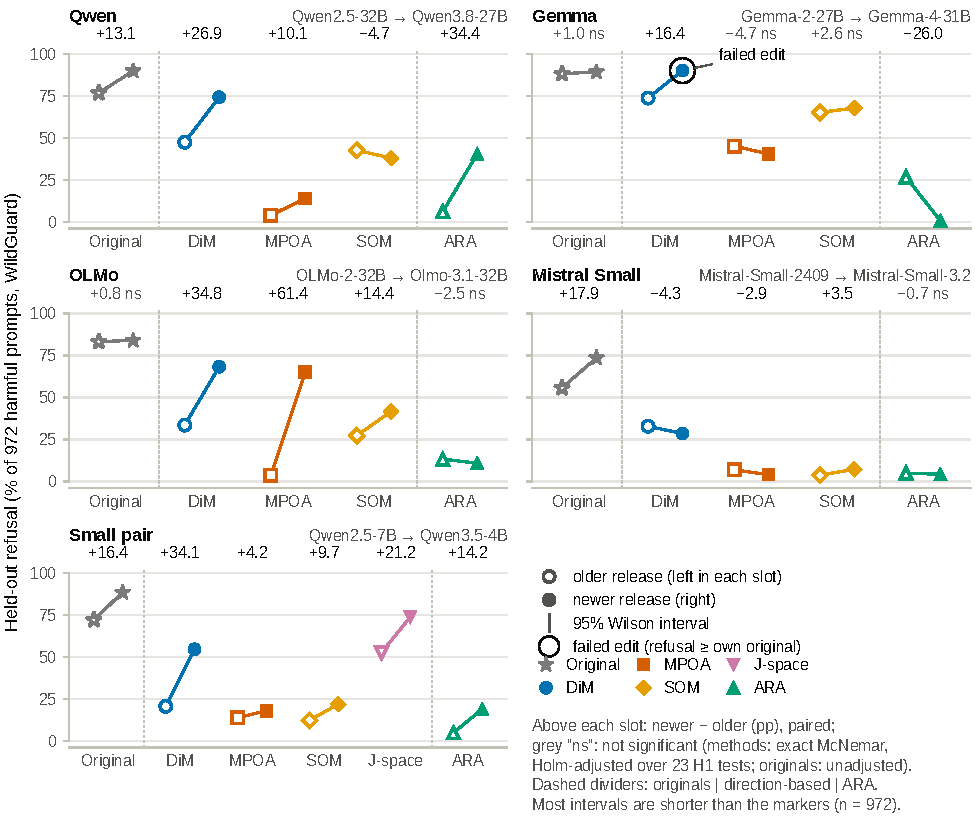
\includegraphics[width=\textwidth]{figures/fig10_heldout_generation_effect.pdf}
\caption{\textbf{Held-out, judged refusal of the original and refusal-removed models, older vs newer release.} Each panel is one pair; each slot is one condition: the unedited originals (grey star), the direction-based methods (DiM, MPOA, SOM; J-space on the small pair only) and, right of the second dashed divider, the optimisation-based ARA. Within a slot the older release (left, hollow marker) is joined to the newer one (right, filled marker). The value is the share of the 972 harmful held-out prompts whose response WildGuard labels a refusal; bars are Wilson 95\% intervals. The number above a slot is the paired generation effect (newer minus older, percentage points), printed in grey with ``ns'' where it is not significant. Significance for the methods is Holm-adjusted (exact McNemar, Holm over the 23 H1 tests); significance for the originals is unadjusted (exact McNemar), because they are the baseline rather than an H1 test. The ring marks a failed edit, a selected model whose held-out refusal is at or above its own original's (Gemma-4-31B DiM). Each modified model is the dev-set selection of its cell (fewest dev keyword refusals at first-token KL $\le$ 0.1, seed 1).}
\label{fig:heldout-generation}
\end{figure*}
% caption: paper/figures/captions.md (fig10_heldout_generation_effect); 2026-11-08 (REV-02): pointer sentences and the
% repeated failed-edit rates removed from the caption (rates in tab:h1-heldout and Appendix app:moved-results).

% Auto-generated by scripts/analysis/make_hypothesis_tables.py at 2026-11-07T00:42:20Z -- do not edit by hand.
% src: results/analysis/h1h2_cells.csv, h1h2_generation_effects.csv, h1h2_tests.csv (judge wg; subsets all and excl_advbench); seednoise_flags.csv, seednoise_sigma.csv

\begin{table*}[t]
\centering\footnotesize
\setlength{\tabcolsep}{3.6pt}
\caption{Held-out residual refusal of the older and newer model of each pair (H1). Rates: share of the 972
harmful held-out prompts whose response WildGuard labels a refusal, with Wilson 95\% intervals. Difference:
newer minus older model in percentage points (pp) with Newcombe 95\% intervals; $b$/$c$: prompts refused only
by the older / only by the newer model (exact McNemar test); $p_\mathrm{Holm}$: Holm over the 23 tests of the
H1 family (21 pair $\times$ method tests and two pooled terms); $^{u}$for the originals the unadjusted McNemar $p$
is given, as they are the baseline rather than an H1 test. Baseline-adjusted: the method's generation effect minus
that of the originals, pp [95\% CI]. Each modified model is the dev-set selection of its cell (first-token KL
$\le 0.1$, seed~1). $^{a}$Not significant after Holm when the 44 prompts that overlap the search prompts are
excluded. $^{b}$Failed edit: held-out refusal at or above the model's own original.
$^{s}$Seed noise: ``exceeds'' if $|$new $-$ old$|$ is larger than 25.9~pp, twice the SD (12.9~pp) of an older-minus-newer difference between two independently optimised cells, otherwise ``within'' (5 of 16 exceed); the per-cell run-to-run SD, 9.2~pp [6.4, 16.1], is estimated from the seed-1 versus seed-2 held-out refusal of the ten small-pair cells (\S\ref{sec:res-h1}) and assumed to transfer to the main pairs. Not given for the small pair, whose replicate is the source of the estimate (Figure~\ref{fig:seed-heldout}).}
\label{tab:h1-heldout}
\begin{tabular}{@{}llllrlll@{}}
\toprule
Condition & Older, \% & Newer, \% & New $-$ old, pp & $b$/$c$ & $p_\mathrm{Holm}$ & Baseline-adj., pp & Seed \\
 & [95\% CI] & [95\% CI] & [95\% CI] & & & [95\% CI] & noise$^{s}$ \\
\midrule
\multicolumn{8}{l}{\emph{Qwen: Qwen2.5-32B $\to$ Qwen3.8-27B}} \\
Original & 76.8 [74.1, 79.4] & 89.9 [87.9, 91.7] & +13.1 [+10.9, +15.4] & 6/133 & $<$0.001$^{u}$ & -- & -- \\
DiM & 47.4 [44.3, 50.6] & 74.3 [71.4, 76.9] & +26.9 [+23.8, +29.8] & 17/278 & $<$0.001 & +13.7 [+10.1, +17.1] & exceeds \\
MPOA & 3.9 [2.9, 5.3] & 14.0 [12.0, 16.3] & +10.1 [+7.8, +12.5] & 23/121 & $<$0.001 & $-$3.1 [$-$6.3, +0.2] & within \\
SOM & 42.7 [39.6, 45.8] & 38.0 [35.0, 41.1] & $-$4.7 [$-$8.0, $-$1.4] & 157/111 & 0.041$^{a}$ & $-$17.8 [$-$21.5, $-$14.2] & within \\
ARA & 6.1 [4.7, 7.8] & 40.4 [37.4, 43.5] & +34.4 [+31.2, +37.5] & 11/345 & $<$0.001 & +21.3 [+17.1, +25.4] & exceeds \\
\midrule
\multicolumn{8}{l}{\emph{Gemma: Gemma-2-27B $\to$ Gemma-4-31B}} \\
Original & 88.3 [86.1, 90.1] & 89.3 [87.2, 91.1] & +1.0 [$-$1.4, +3.5] & 69/79 & 0.460$^{u}$ & -- & -- \\
DiM & 73.8 [70.9, 76.4] & 90.1 [88.1, 91.8]$^{b}$ & +16.4 [+13.5, +19.3] & 35/194 & $<$0.001 & +15.3 [+13.0, +17.8] & within \\
MPOA & 45.2 [42.1, 48.3] & 40.4 [37.4, 43.5] & $-$4.7 [$-$8.6, $-$0.9] & 206/160 & 0.093 & $-$5.8 [$-$9.7, $-$1.7] & within \\
SOM & 65.2 [62.2, 68.2] & 67.8 [64.8, 70.7] & +2.6 [$-$1.1, +6.2] & 151/176 & 0.369 & +1.5 [$-$1.9, +4.9] & within \\
ARA & 26.6 [24.0, 29.5] & 0.6 [0.3, 1.3] & $-$26.0 [$-$28.9, $-$23.3] & 253/0 & $<$0.001 & $-$27.1 [$-$30.3, $-$23.6] & exceeds \\
\midrule
\multicolumn{8}{l}{\emph{OLMo: OLMo-2-32B $\to$ Olmo-3.1-32B}} \\
Original & 83.2 [80.8, 85.4] & 84.1 [81.6, 86.2] & +0.8 [$-$0.6, +2.2] & 19/27 & 0.302$^{u}$ & -- & -- \\
DiM & 33.5 [30.6, 36.6] & 68.3 [65.3, 71.2] & +34.8 [+31.5, +37.9] & 14/352 & $<$0.001 & +34.0 [+30.5, +37.6] & exceeds \\
MPOA & 3.6 [2.6, 5.0] & 65.0 [62.0, 68.0] & +61.4 [+58.2, +64.4] & 2/599 & $<$0.001 & +60.6 [+57.1, +64.1] & exceeds \\
SOM & 27.3 [24.6, 30.1] & 41.7 [38.6, 44.8] & +14.4 [+11.5, +17.3] & 45/185 & $<$0.001 & +13.6 [+10.4, +16.7] & within \\
ARA & 13.3 [11.3, 15.5] & 10.8 [9.0, 12.9] & $-$2.5 [$-$4.6, $-$0.3] & 67/43 & 0.111 & $-$3.3 [$-$5.8, $-$0.9] & within \\
\midrule
\multicolumn{8}{l}{\emph{Mistral Small: Mistral-Small-2409 $\to$ Mistral-Small-3.2}} \\
Original & 55.7 [52.6, 58.8] & 73.6 [70.7, 76.2] & +17.9 [+15.2, +20.6] & 21/195 & $<$0.001$^{u}$ & -- & -- \\
DiM & 32.8 [29.9, 35.8] & 28.5 [25.7, 31.4] & $-$4.3 [$-$7.4, $-$1.2] & 141/99 & 0.048$^{a}$ & $-$22.2 [$-$26.1, $-$18.4] & within \\
MPOA & 6.9 [5.5, 8.7] & 4.0 [2.9, 5.4] & $-$2.9 [$-$4.7, $-$1.2] & 51/23 & 0.014 & $-$20.8 [$-$24.0, $-$17.7] & within \\
SOM & 3.7 [2.7, 5.1] & 7.2 [5.7, 9.0] & +3.5 [+1.7, +5.3] & 22/56 & 0.001 & $-$14.4 [$-$17.7, $-$11.1] & within \\
ARA & 4.9 [3.7, 6.5] & 4.2 [3.1, 5.7] & $-$0.7 [$-$2.1, +0.6] & 23/16 & 0.369 & $-$18.6 [$-$21.6, $-$15.7] & within \\
\midrule
\multicolumn{8}{l}{\emph{Small pair: Qwen2.5-7B $\to$ Qwen3.5-4B}} \\
Original & 72.1 [69.2, 74.8] & 88.5 [86.3, 90.3] & +16.4 [+13.9, +18.9] & 11/170 & $<$0.001$^{u}$ & -- & -- \\
DiM & 20.6 [18.2, 23.2] & 54.6 [51.5, 57.7] & +34.1 [+30.5, +37.5] & 43/374 & $<$0.001 & +17.7 [+13.5, +21.8] & -- \\
MPOA & 13.8 [11.8, 16.1] & 18.0 [15.7, 20.5] & +4.2 [+1.6, +6.9] & 66/107 & 0.018 & $-$12.1 [$-$15.7, $-$8.3] & -- \\
SOM & 12.2 [10.3, 14.5] & 21.9 [19.4, 24.6] & +9.7 [+6.9, +12.4] & 50/144 & $<$0.001 & $-$6.7 [$-$10.4, $-$3.0] & -- \\
J-space & 52.6 [49.4, 55.7] & 73.8 [70.9, 76.4] & +21.2 [+18.1, +24.3] & 37/243 & $<$0.001 & +4.8 [+1.3, +8.3] & -- \\
ARA & 4.7 [3.6, 6.3] & 18.9 [16.6, 21.5] & +14.2 [+11.6, +16.9] & 24/162 & $<$0.001 & $-$2.2 [$-$6.0, +1.6] & -- \\
\bottomrule
\end{tabular}
\end{table*}


\paragraph{Baseline.} The newer Qwen, Mistral Small and small-pair originals
already refused more than their predecessors (+13.1, +17.9 and +16.4~pp); the
Gemma and OLMo originals did not. Relative to this difference the
direction-based effect was near zero in Qwen and the small pair, negative in
Mistral Small and unchanged in Gemma and OLMo (Table~\ref{tab:pair-effects});
the two scales of this adjustment disagreed in sign for 3 of 21 pair $\times$
method cells (Appendix~\ref{app:kl-cap}, Table~\ref{tab:scales}). As a
scale-free alternative, the share of the prompts refused by a model's own
original that the edited model still refused rose on the newer model by
+43.4~pp in OLMo (95\% interval with run-to-run variance [+25.7, +61.1]) and
+13.5~pp in the small pair ([$-$1.9, +28.9]) after direction-based removal, and
changed by $-$6.6 to +6.0~pp in the other pairs, none of which excluded zero
(Table~\ref{tab:retention}).
% 2026-11-08 ARS re-review revision (NEW-5): src: results/analysis/revision_rr_retention.csv (direction class lo_total / hi_total:
% src: olmo +25.7 / +61.1, qwen-small -1.9 / +28.9, qwen -11.7 / +23.7, gemma -13.8 / +21.7, mistral -24.3 / +11.1;
% src: scripts/analysis/revision_rr_extra.py, sigma_ret 10.96 pp from the 10 small-pair seed pairs).
% src: results/analysis/h1h2_generation_effects.csv (original rows); review_sel_pair_effects.csv (adjusted); review_sel_scales.csv
% src: (sign differs in 3 of 21); (2026-11-08 revision, REV-19) revision_retention.csv (direction class: olmo +43.4 [+41.0, +45.7],
% src: qwen-small +13.5, qwen +6.0, gemma +4.0, mistral -6.6; prompt-bootstrap intervals, prompt sampling only).

\paragraph{Item source.} The per-pair verdicts depended in part on where the
prompts came from (Table~\ref{tab:pair-source}). The code-as-weapon bank (200
of the 972 prompts), compiled by the author, carried 52\% of the mean
originals' difference of the four main pairs. Gemma's direction-based increase
came entirely from it: +49.3~pp on the code items against $-$6.8~pp on the
public sets. The OLMo direction-based increase, the Mistral Small null and the
sign of the Gemma and OLMo H2 contrasts held on both sources; the Gemma ARA
decrease lay in the public sets (the code items were near the floor), and the
Qwen H2 contrast was positive on the public sets (+30.3~pp) and near zero on
the code items ($-$1.8~pp).
% src: results/analysis/review_out_c2_pair_class.csv (item_subset public4 / code_weapon: rd_dir_raw gemma -6.8 / +49.3, olmo
% src: +45.2 / +4.8, mistral -1.6 / +0.2; rd_ara_raw gemma -32.4 / -1.5; rd_h2_rd qwen +30.3 / -1.8, gemma -25.6 / -50.8, olmo
% src: -48.3 / -4.8); review_out_c2_originals_decomposition.csv (mean of 4 main pairs, code share 0.52 [0.44, 0.60]).

% Hand-written 2026-11-08 (ARS revision, REV-13): per-pair class effects by item source in the main text.
% src: results/analysis/review_out_c2_pair_class.csv (item_subset public4 and code_weapon; judge wg; columns rd_orig,
% src: rd_dir_raw, rd_ara_raw, rd_h2_rd with _lo / _hi; x 100), written by scripts/analysis/review_outcomes.py (C2);
% src: item-bootstrap 95% intervals (prompt sampling only). Code items: 199 for Qwen and Mistral (one missing WildGuard label).
\begin{table*}[t]
\centering\scriptsize
\setlength{\tabcolsep}{2.4pt}
\caption{Per-pair generation effects (newer minus older model, pp) by item source: the four public sets (JailbreakBench,
XSTest unsafe, StrongREJECT, HarmBench; 772 prompts) and the author-compiled code-as-weapon bank (200 prompts).
Originals: unedited models. Direction: mean of the direction-based methods. H2: ARA minus direction. Item-bootstrap
95\% intervals, prompt sampling only (run-to-run variance not added). Many edited models refused none of the code
items, so effects on them are bounded near zero. All-item values are in Table~\ref{tab:pair-effects}; pooled log-odds
by item set in Table~\ref{tab:item-source}.}
\label{tab:pair-source}
\resizebox{\textwidth}{!}{%
\begin{tabular}{@{}lllllllll@{}}
\toprule
 & \multicolumn{2}{c}{Originals} & \multicolumn{2}{c}{Direction} & \multicolumn{2}{c}{ARA} & \multicolumn{2}{c}{H2 contrast} \\
\cmidrule(lr){2-3}\cmidrule(lr){4-5}\cmidrule(lr){6-7}\cmidrule(l){8-9}
Pair & Public & Code & Public & Code & Public & Code & Public & Code \\
\midrule
Qwen & +5.3 [+3.5, +7.1] & +43.2 [+36.5, +50.5] & +11.0 [+8.8, +13.3] & +9.4 [+6.5, +12.4] & +41.3 [+37.6, +45.1] & +7.5 [+4.0, +11.5] & +30.3 [+25.9, +34.6] & $-$1.8 [$-$5.5, +2.0] \\
Gemma & $-$5.7 [$-$7.5, $-$4.0] & +27.0 [+18.0, +36.0] & $-$6.8 [$-$9.5, $-$4.4] & +49.3 [+43.7, +55.0] & $-$32.4 [$-$35.8, $-$29.0] & $-$1.5 [$-$3.5, 0.0] & $-$25.6 [$-$29.3, $-$21.9] & $-$50.8 [$-$56.3, $-$45.2] \\
OLMo & $-$0.3 [$-$1.6, +1.0] & +5.0 [+0.5, +9.5] & +45.2 [+42.8, +47.5] & +4.8 [+2.7, +7.2] & $-$3.1 [$-$5.7, $-$0.4] & 0.0 [0.0, 0.0] & $-$48.3 [$-$51.6, $-$44.9] & $-$4.8 [$-$7.2, $-$2.7] \\
Mistral Small & +20.5 [+17.2, +23.7] & +8.0 [+4.5, +12.1] & $-$1.6 [$-$3.5, +0.2] & +0.2 [0.0, +0.5] & $-$0.9 [$-$2.5, +0.6] & 0.0 [0.0, 0.0] & +0.7 [$-$1.6, +3.0] & $-$0.2 [$-$0.5, 0.0] \\
Small pair & +9.5 [+7.1, +11.9] & +43.0 [+36.0, +50.0] & +20.2 [+17.9, +22.7] & +5.9 [+4.1, +7.6] & +17.7 [+14.6, +21.0] & +0.5 [0.0, +1.5] & $-$2.5 [$-$6.1, +1.2] & $-$5.4 [$-$7.2, $-$3.5] \\
\bottomrule
\end{tabular}}
\end{table*}


% ------------------------------------------------------------
\subsection{H2: Generation \texorpdfstring{$\times$}{x} Edit Class}
\label{sec:res-h2}

ARA, a rank-50 per-module edit, lost less effectiveness on the newer model
than the low-rank direction-based edits in the Gemma ($-$30.8~pp) and OLMo
($-$39.3~pp) pairs, more in the Qwen pair (+23.6~pp), and about as much in
Mistral Small and the small pair (Tables~\ref{tab:pair-effects}
and~\ref{tab:h2-contrasts}). Each per-pair contrast rests on a single ARA cell.
With constant run-to-run variance, only the Gemma and OLMo contrasts excluded
zero; with the refusal-level variance, only OLMo did. The Qwen contrast is
therefore indeterminate: its interval with run-to-run variance included zero
($-$5.9 to +53.1~pp). Pooled with the pair as the unit, the contrast was
$-$11.5~pp [$-$57.6, +34.6]. The planned mixed model gave the same signs
(Appendix~\ref{app:rr-tables}, Table~\ref{tab:h2-vb}).
% 2026-11-08 ARS re-review revision (REV-17, REV-20): Qwen H2 called indeterminate (review_sel_pair_effects.csv, qwen H2 pp
% src: lo_total -0.0588, hi_total 0.5314); VB column moved to tab:h2-vb (t15_h2_vb.tex; signs as GEE in every row).
% src: results/analysis/review_sel_pair_effects.csv (H2 contrast pp, lo_total / hi_total); revision_sigma_pair_verdicts.csv
% src: (H2 excl0_level_point: olmo only); review_sel_pair_meta.csv (H2 pp prompt sampling only: -11.49 [-57.63, 34.65]);
% src: sections/08b_setup_details.tex (ARA rank 50; DiM 1, MPOA/J-space 3, SOM 6).

\paragraph{KL cap and budget.} The KL cap bound in all 8 ARA runs but in 15 of
the 24 direction-based runs. Restricted to the direction-based units in which
it bound in both cells (Qwen DiM; Gemma DiM, MPOA and SOM; Mistral Small DiM;
none in OLMo), the H2 contrast was +7.5~pp [$-$28.6, +43.7] in Qwen,
$-$30.8~pp [$-$60.2, $-$1.3] in Gemma and +3.6~pp [$-$32.4, +39.6] in Mistral
Small, and pooled $-$8.5~pp [$-$62.5, +45.5]. Away from the selected budget
only dev-set keyword counts exist, and both checks below use them. Their
validity for H2 is limited: at the selected budget, the dev ARA generation
effects had the opposite sign to the held-out judged ARA effects in three of
the four main pairs (Appendix~\ref{app:kl-budgets}), so these checks show how
stable the dev-set contrast is, not the held-out one. On them the direction-based generation
effects kept their sign at every budget from 0.1 to 1.0 in all four main
pairs, whereas the H2 contrast changed sign with the budget in three of them
(Gemma above KL~$=0.1$; OLMo and Mistral Small below it). On the area under
the refusal--KL front, a budget-free summary, the contrast was in the
predicted direction but within run-to-run variation in Gemma and OLMo and
opposite, beyond it, in Qwen and Mistral Small (Appendix~\ref{app:kl-budgets},
Table~\ref{tab:kl-budgets}).
% src: results/analysis/review_sel_kl_summary.csv (15 of 24; 8 of 8); (2026-11-08 revision, REV-16) revision_h2_sensitivity.csv
% src: (cap-bound direction units only: qwen +7.5 [-28.6, +43.7], gemma -30.8 [-60.2, -1.3], mistral +3.6 [-32.4, +39.6]; olmo not
% src: estimable); revision_h2_sensitivity_meta.csv (pooled cap-bound, prompt + seed: -8.5 [-62.5, +45.5]);
% src: (REV-16, REV-32) revision_kl_budget_effects.csv (direction class sign_as_at_0.1 = 1 for t0.2, t0.5, t1 in all 4 main pairs;
% src: H2 gemma +7.3 at t0.1, -18.7 / -29.0 / -29.0 at t0.2 / t0.5 / t1; olmo +12.7 at t0.05, -26.0 at t0.1; mistral -4.0 at t0.05,
% src: +8.0 at t0.1; AUC H2 qwen +44.3*, gemma -7.9, olmo -6.0, mistral +17.1*; * beyond 1.96 run-to-run SE).
% 2026-11-08 ARS re-review revision (NEW-8): validity limit of the dev-based checks stated in the main text.
% src: revision_kl_budget_effects.csv (ara sign as held-out in 1 of 4 main pairs at every quantity); sections/08i_revision_details.tex
% src: (app:kl-budgets: "opposite sign to the held-out ARA effects in three of the four main pairs").

\paragraph{ARA cells.} Three properties of the ARA cells bear on these
contrasts (Appendix~\ref{app:moved-results}): the four ARA exports refitted on
a different GPU from the search (Qwen and Gemma pairs) drifted more on dev
re-score than those refitted on the search GPU; the Gemma-4-31B ARA export,
behind the largest contrast, re-scored above the KL cap (0.107); and a public
ARA model of Qwen3.8-27B built with the same defaults refused 26.4\% of the
held-out prompts, against 40.4\% for the ARA model selected here, on which the
reversed Qwen estimate rests. Without the failed Gemma-4-31B DiM edit, the Gemma
contrast was $-$24.9~pp [$-$56.2, +6.3].
% src: results/analysis/review_sel_export_drift.csv, review_sel_export_tests.csv (Fisher p 0.029; Gemma-4-31B KL 0.1070);
% src: final_community_vs_selected.csv (hereticorg-ara 0.2644 vs qwen3.8-27b__ara 0.4043); (2026-11-08 revision, REV-27)
% src: revision_h2_sensitivity.csv ("Gemma without the failed Gemma-4-31B DiM edit", H2 contrast -24.9 [-56.2, +6.3]).

% 2026-11-08 ARS re-review revision (REV-20): t5b = t5 without the VB column (scripts/analysis/revision_rr_extra.py).
% Auto-generated by scripts/analysis/revision_rr_extra.py at 2026-11-09T04:36Z -- do not edit by hand.
% src: paper/tables/t5_h2_contrasts.tex (make_hypothesis_tables.py; results/analysis/h1h2_h2_contrasts.csv,
% h1h2_tests.csv, h1h2_models.csv); columns split only, no number changed.
\begin{table*}[t]
\centering\footnotesize
\setlength{\tabcolsep}{3pt}
\caption{Generation $\times$ method-class interaction (H2) on held-out WildGuard refusal. ARA and direction
mean: generation effects (newer minus older model, pp) of ARA and of the mean of the direction-based methods
(DiM, MPOA, SOM; on the small pair also J-space). RD contrast: ARA minus direction mean, pp, item-bootstrap
95\% interval. GEE: generation $\times$ class interaction in log-odds (exchangeable, clustered by prompt) with
95\% interval; $p_\mathrm{Holm}$ over the six H2 tests. Pooled (main): the four main-study pairs. All
intervals here reflect prompt sampling only; the per-pair intervals with run-to-run variance are in
Table~\ref{tab:pair-effects}, and the planned mixed-model estimates in Table~\ref{tab:h2-vb}. H2 predicts a
negative interaction (ARA loses less effectiveness on the newer model); sign vs.\ H2: GEE interaction
significant after Holm and negative (predicted) or positive (opposite), or not significant (n.s.).
$^{c}$The RD contrast and the log-odds interaction have opposite signs.}
\label{tab:h2-contrasts}
\begin{tabular}{lrrllll}
\toprule
Pair & ARA, & Direction & RD contrast, pp & GEE, log-odds & $p_\mathrm{Holm}$ & Sign \\
 & pp & mean, pp & [95\% CI] & [95\% CI] & & vs.\ H2 \\
\midrule
Qwen & +34.4 & +10.7 & +23.6 [+19.9, +27.1] & +1.89 [+1.61, +2.16] & $<$0.001 & opposite \\
Gemma & $-$26.0 & +4.7 & $-$30.8 [$-$34.0, $-$27.5] & $-$4.27 [$-$5.07, $-$3.47] & $<$0.001 & predicted \\
OLMo & $-$2.5 & +36.9 & $-$39.3 [$-$42.2, $-$36.4] & $-$1.87 [$-$2.08, $-$1.65] & $<$0.001 & predicted \\
Mistral Small & $-$0.7 & $-$1.2 & +0.5 [$-$1.4, +2.4] & $-$0.06 [$-$0.37, +0.25] & 0.696 & n.s. \\
Small pair & +14.2 & +17.3 & $-$3.1 [$-$6.0, $-$0.1] & +0.76 [+0.46, +1.06] & $<$0.001 & opposite$^{c}$ \\
\midrule
Pooled (main) & -- & -- & -- & $-$0.50 [$-$0.62, $-$0.38] & $<$0.001 & predicted \\
\bottomrule
\end{tabular}
\end{table*}


% ------------------------------------------------------------
\subsection{H3: Keyword Counts versus an Automatic Judge}
\label{sec:res-h3}

H3's prediction that keyword matching would count fewer refusals than the
judge was not supported at any window (Table~\ref{tab:h3-windows},
Figure~\ref{fig:judge-agreement}). At the 100-token window that Heretic scores,
an exploratory window added after the held-out results were known, keyword
matching and WildGuard agreed on average over the 42 ablated models (+0.5~pp
[$-$1.0, +1.9]) but differed by 7.0~pp per model on average, significantly in
25 models and in both directions. Over the full response keyword matching
counted more refusals (+8.4~pp [+6.9, +10.0]), mainly through markers after
the first 100 tokens. In the main study the gap was larger for ARA and on the
newer models with the prompt as the unit, but not with the model as the unit
(Table~\ref{tab:h3-gap}). Keyword--WildGuard agreement fell from
$\kappa=0.73$ in the originals to 0.40 (main study) after ablation, whereas
the two LLM judges agreed at 0.82.
% src: results/analysis/review_out_c4_gap_pooled.csv (kw100_vs_wg ablated_primary +0.5 [-1.0, +1.9]); review_out_summary.md C4
% src: (14 higher + 11 lower Holm-significant of 42); (2026-11-08 revision, REV-39) revision_kw_gap_abs.csv (kw100_vs_wg mean |gap|
% src: 7.0 pp); h3_gap_pooled.csv (kw_vs_wg +8.4 [+6.9, +10.0]); review_out_c4_models.csv (GEE class / generation /
% src: interaction p_holm < 0.001; OLS p 0.17 / 0.28); h3_agreement_pairs.csv (0.73, 0.40, WildGuard vs Qwen3Guard 0.82).

% Hand-written 2026-11-06 (review revision; reviewer concern C4). Not generated by make_hypothesis_tables.py.
% src: 512-token (full-response) columns = tables/t6_h3_gap.tex (results/analysis/h3_gap_pooled.csv kw_vs_wg,
% src: kw_vs_wg_complete_only, kw_vs_wg_capped_only); 256-token gap = tables in sections/08e_truncation256.tex
% src: (results/analysis/trunc256_pooled.csv kw256_vs_wg256[_complete_only|_capped_only]); 100-token columns =
% src: results/analysis/review_out_c4_gap_pooled.csv (subset harmful_all; variant kw100_vs_wg, kw100_vs_wg_complete_only,
% src: kw100_vs_wg_capped_only; rate1 = kw100 %, rate2 = WG %) = review_out_summary.md C4 pooled table.
% src: Per-cell counts (caption): review_out_summary.md C4 "Per evaluated model" (kw_vs_wg 34/7 (24/3 Holm);
% src: kw100_vs_wg 24/18 (14/11 Holm)), from review_out_c4_gap_cells.csv.
\begin{table*}[t]
\centering\footnotesize
\setlength{\tabcolsep}{2.8pt}
\caption{Keyword matching versus WildGuard on the same held-out responses to the 972 harmful prompts, by keyword window
(H3). Kw: refusal rate by Heretic's 33 markers in the full response (at most 512 tokens) or in its first 100 tokens,
the window Heretic scores during search; WG: WildGuard refusal on the full response. Gap: keyword minus WildGuard, pp,
with prompt-cluster bootstrap 95\% intervals; 512 and 100 tokens: keyword on that window against WildGuard on the full
response; 256 tokens: both on the first 256 tokens (Appendix~\ref{app:trunc256}). H3 predicted a negative gap. Over
the 42 ablated models the gap was positive in 34 models (24 Holm-significant) and negative in 7 (3) at 512 tokens, and
positive in 24 (14) and negative in 18 (11) at 100 tokens. Ablated: the 42 seed-1 models selected from the primary runs;
cap: the 512-token generation limit.}
\label{tab:h3-windows}
\begin{tabular}{@{}lrrrrlll@{}}
\toprule
 & & \multicolumn{2}{c}{Kw, \%} & & \multicolumn{3}{c}{Gap, pp [95\% CI]} \\
\cmidrule(lr){3-4}\cmidrule(lr){6-8}
Models & Cells & 512 & 100 & WG, \% & 512 tokens & 256 tokens & 100 tokens \\
\midrule
Originals & 10 & 82.8 & 80.9 & 80.2 & +2.6 [+1.8, +3.4] & +1.6 [+0.8, +2.4] & +0.7 [$-$0.1, +1.5] \\
\midrule
Ablated (seed 1), all & 42 & 39.9 & 32.0 & 31.5 & +8.4 [+6.9, +10.0] & +3.8 [+2.4, +5.2] & +0.5 [$-$1.0, +1.9] \\
\quad main study & 32 & 42.0 & 33.8 & 32.3 & +9.8 [+8.2, +11.3] & +4.9 [+3.5, +6.4] & +1.5 [+0.0, +2.9] \\
\quad small pair & 10 & 33.3 & 26.5 & 29.1 & +4.2 [+2.5, +5.9] & +0.4 [$-$1.4, +2.0] & $-$2.6 [$-$4.3, $-$0.9] \\
\quad responses ending before the cap & 42 & 51.2 & 42.1 & 52.4 & $-$1.2 [$-$3.2, +0.9] & $-$5.6 [$-$7.6, $-$3.8] & $-$10.4 [$-$12.2, $-$8.6] \\
\quad responses truncated at the cap & 42 & 29.1 & 22.4 & 11.4 & +17.7 [+16.2, +19.3] & +13.0 [+11.5, +14.4] & +11.0 [+9.7, +12.4] \\
\midrule
$\gamma$-MPOA control & 4 & 47.0 & 38.7 & 29.9 & +17.1 [+14.9, +19.4] & +12.0 [+9.9, +14.0] & +8.8 [+6.8, +10.9] \\
Community releases & 8 & 22.9 & 17.3 & 6.4 & +16.5 [+15.2, +17.8] & +13.6 [+12.4, +14.8] & +11.0 [+9.8, +12.1] \\
Seed-2 replicates (small pair) & 10 & 32.8 & 26.4 & 29.2 & +3.5 [+2.0, +5.0] & +0.0 [$-$1.5, +1.4] & $-$2.9 [$-$4.3, $-$1.5] \\
\midrule
All judged models & 74 & 43.3 & 36.6 & 35.0 & +8.3 [+7.0, +9.6] & +4.5 [+3.3, +5.7] & +1.7 [+0.5, +2.8] \\
\bottomrule
\end{tabular}
\end{table*}


% Table before the figure float so that it is placed next to sec:res-h3 (2026-11-06 fact-check pass)
% Auto-generated by scripts/analysis/make_hypothesis_tables.py at 2026-11-07T00:42:20Z -- do not edit by hand.
% src: results/analysis/h3_gap_pooled.csv (subset harmful_all), h3_agreement_pairs.csv (subset harmful, pooled, kw vs wg)

\begin{table}[t]
\centering\footnotesize
\setlength{\tabcolsep}{3pt}
\caption{Keyword matching versus WildGuard on the same held-out responses to the 972 harmful prompts (H3).
Keyword: any of Heretic's 33 refusal markers in the full response (at most 512 tokens). Gap: keyword minus
WildGuard refusal rate, pp, with prompt-cluster bootstrap 95\% interval (H3 predicted a negative gap). kw/WG only: responses counted
as refusals by keyword matching only / by WildGuard only. $\kappa$: Cohen's kappa with prompt-bootstrap 95\%
interval. Ablated: the 42 seed-1 models selected from the primary runs.}
\label{tab:h3-gap}
\begin{tabular}{lrrrrlrl}
\toprule
Models & Cells & Responses & Kw, \% & WG, \% & Gap, pp [95\% CI] & kw/WG only & $\kappa$ [95\% CI] \\
\midrule
Originals & 10 & 9{,}718 & 82.8 & 80.2 & +2.6 [+1.8, +3.4] & 531/277 & 0.73 [0.70, 0.75] \\
\midrule
Ablated (seed 1), all & 42 & 40{,}824 & 39.9 & 31.5 & +8.4 [+6.9, +10.0] & 7{,}503/4{,}059 & 0.39 [0.37, 0.41] \\
\quad main study & 32 & 31{,}104 & 42.0 & 32.3 & +9.8 [+8.2, +11.3] & 5{,}897/2{,}859 & 0.40 [0.39, 0.42] \\
\quad small pair & 10 & 9{,}720 & 33.3 & 29.1 & +4.2 [+2.5, +5.9] & 1{,}606/1{,}200 & 0.33 [0.31, 0.35] \\
\quad responses ending before the cap & 42 & 20{,}011 & 51.2 & 52.4 & $-$1.2 [$-$3.2, +0.9] & 2{,}998/3{,}240 & -- \\
\quad responses truncated at 512 tokens & 42 & 20{,}813 & 29.1 & 11.4 & +17.7 [+16.2, +19.3] & 4{,}505/819 & -- \\
\midrule
$\gamma$-MPOA control & 4 & 3{,}888 & 47.0 & 29.9 & +17.1 [+14.9, +19.4] & 1{,}038/372 & 0.26 [0.23, 0.29] \\
Community releases & 8 & 7{,}776 & 22.9 & 6.4 & +16.5 [+15.2, +17.8] & 1{,}475/192 & 0.18 [0.16, 0.21] \\
Seed-2 replicates (small pair) & 10 & 9{,}720 & 32.8 & 29.2 & +3.5 [+2.0, +5.0] & 1{,}351/1{,}010 & 0.43 [0.41, 0.46] \\
\midrule
All judged models & 74 & 71{,}926 & 43.3 & 35.0 & +8.3 [+7.0, +9.6] & 11{,}898/5{,}910 & 0.48 [0.47, 0.50] \\
\bottomrule
\end{tabular}
\end{table}


\begin{figure*}[!htbp]
\centering
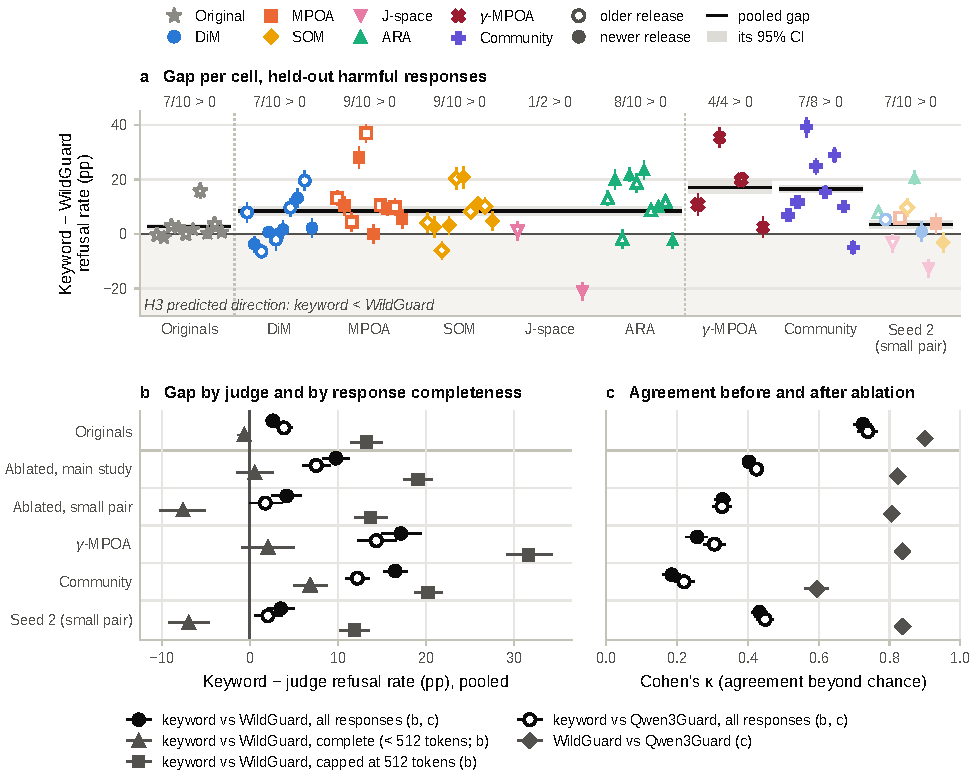
\includegraphics[width=\textwidth]{figures/fig11_judge_agreement.pdf}
\caption{\textbf{Keyword counts versus two LLM judges on the same held-out responses (H3).} (a) Each marker is one evaluated model (cell): its keyword refusal rate (any of Heretic's 33 refusal markers in the first 100 generated tokens, the window Heretic scores during search) minus its WildGuard refusal rate on the 972 harmful held-out prompts, in percentage points, with a paired 95\% interval (Newcombe). Slots, left to right: the unedited originals, the seed-1 ablated models by method (direction-based, then ARA), $\gamma$-MPOA, public community releases and the small pair's seed-2 replicates (lighter); within a slot the models run in pair order (Qwen, Gemma, OLMo, Mistral Small, small pair), hollow = older, filled = newer release. The black bar and grey band are the pooled gap of the slot group with its 95\% interval; the count above a slot is the number of cells with a positive gap. H3 predicted the shaded region (keyword below the judge). (b) Pooled keyword-minus-WildGuard gap for keyword windows of 100 and 256 tokens and the full response (at most 512 tokens). (c) Cohen's $\kappa$ of the full-response keyword label, with prompt-bootstrap 95\% intervals. No human-labelled audit exists, so the panels show where keyword matching and the judges disagree, not which is correct.}
\label{fig:judge-agreement}
\end{figure*}
% caption: paper/figures/captions.md (fig11_judge_agreement); 2026-11-08 (REV-02, REV-33): "diverge" -> "disagree"; the
% sentence on the gap growing with the window (in the text) removed.

% ------------------------------------------------------------
\subsection{Secondary Outcomes}
\label{sec:res-secondary}

\paragraph{$\gamma$-MPOA control.} Correcting MPOA for the post-norm output
gains (Appendix~\ref{app:setup-methods}) lowered held-out refusal on all four
post-norm models (Figure~\ref{fig:gmpoa-heldout}), more on the newer model of
each pair: by 4.2 and 19.9~pp on Gemma-2-27B and Gemma-4-31B (generation
difference $-$15.6~pp [$-$19.6, $-$11.7]) and by 3.1 and 7.5~pp on OLMo-2-32B
and Olmo-3.1-32B ($-$4.4~pp [$-$6.6, $-$2.2]). With $\gamma$-MPOA in place of
MPOA, the OLMo generation effect remained +57.0~pp and the pooled
prompt-level H2 interaction $-$0.42 log-odds. On Gemma-4-31B and OLMo-2-32B,
$\gamma$-MPOA lost 21.4 and 8.1~pp of mean capability. DiM and SOM were not
corrected.
% src: results/analysis/final_gmpoa_control.csv (vs_mpoa_diff); final_gmpoa_generation.csv (olmo +57.0); final_pooled_robustness.csv
% src: (gamma-MPOA replaces MPOA: -0.42); final_capability.csv (-21.4, -8.1); (2026-11-08 revision, REV-24) revision_h2_sensitivity.csv
% src: (gemma: gMPOA - MPOA older -4.2, newer -19.9, generation difference -15.6 [-19.6, -11.7]; olmo -3.1, -7.5, -4.4 [-6.6, -2.2];
% src: prompt sampling only).

\begin{figure*}[!htbp]
\centering
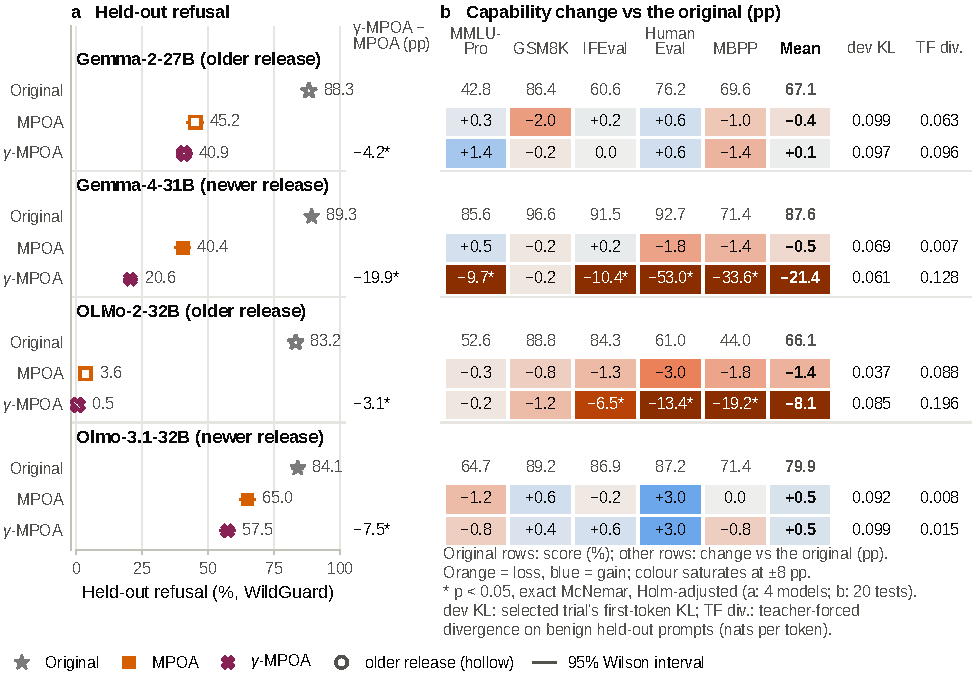
\includegraphics[width=\textwidth]{figures/fig12_gamma_mpoa_heldout.pdf}
\caption{\textbf{$\gamma$-corrected MPOA versus MPOA on the four post-norm models: held-out, judged refusal and capability.} Each block is one model (older or newer release of the Gemma and OLMo pairs) with its unedited original (grey star), the selected MPOA model (vermillion square) and the selected $\gamma$-MPOA model (wine-red cross; MPOA with the edit corrected for the post-norm output gains); hollow markers are the older releases. (a) Share of the 972 harmful held-out prompts whose response WildGuard labels a refusal, with Wilson 95\% intervals; the column on the right is $\gamma$-MPOA minus MPOA (percentage points, paired; * = significant, exact McNemar, Holm over the four models). (b) Change of each benchmark score from the model's own original, in percentage points (orange = loss, blue = gain; the colour saturates at $\pm$8 pp, the printed values are exact; the original's row gives its scores in \%); * marks a $\gamma$-MPOA score that differs from the original's (paired per-item McNemar, Holm over 20 tests). The last two columns are the selected trial's dev first-token KL divergence and the teacher-forced divergence on the 350 benign held-out prompts (nats per token). Single seed; one benchmark item is worth 0.1--0.61 pp.}
\label{fig:gmpoa-heldout}
\end{figure*}
% caption: paper/figures/captions.md (fig12_gamma_mpoa_heldout)

\paragraph{Community releases.} Of eight public abliterations of five of the
checkpoints (Figure~\ref{fig:community}), four refused less than the best
model selected here for the same checkpoint, for example 1.4\% against 14.0\%
on Qwen3.8-27B and 0.7\% against 10.8\% on Olmo-3.1-32B, at teacher-forced
divergences of 0.085--0.151 (best selected models 0.042--0.060) and mean
capability changes within 1~pp.
% src: results/analysis/final_community_vs_selected.csv (rows with ours_is_best_wg; p_holm < 0.001; tf 0.085-0.151 vs 0.042-0.060;
% src: capability -0.94 to -0.15 pp).

\begin{figure*}[!htbp]
\centering
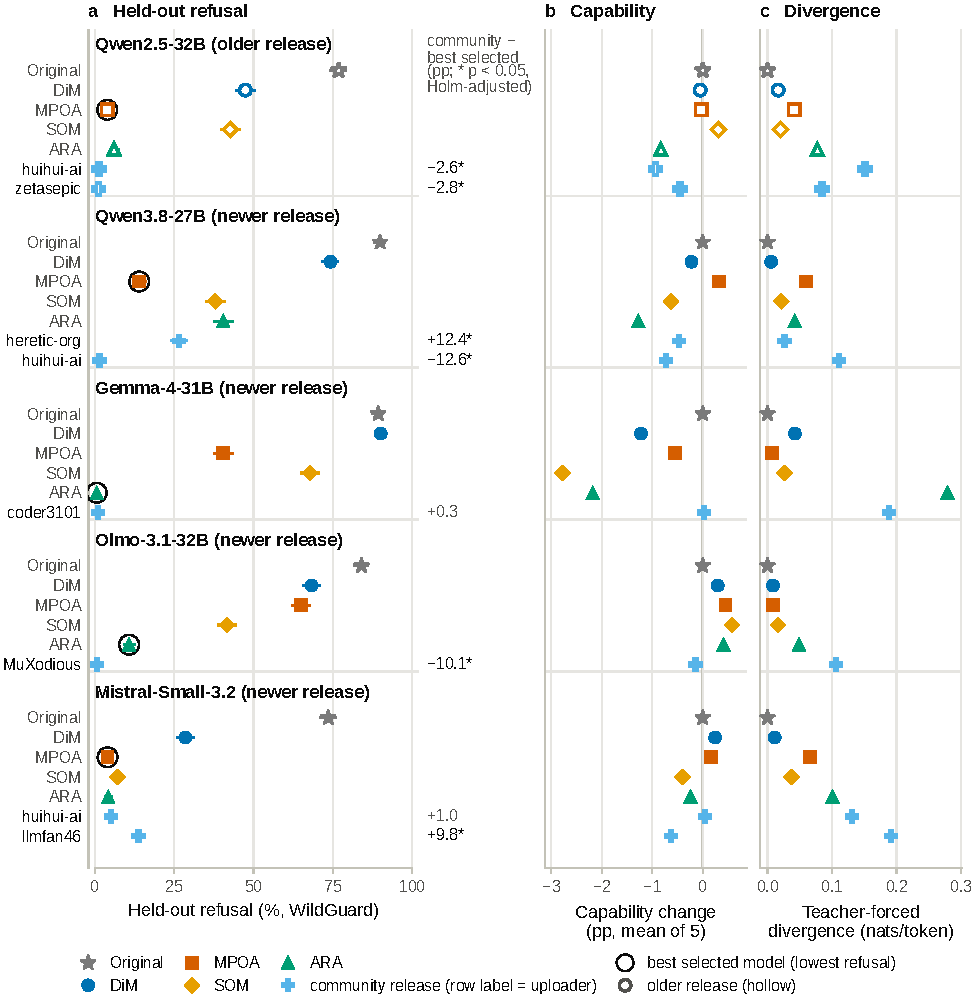
\includegraphics[width=\textwidth]{figures/fig14_community.pdf}
\caption{\textbf{Models selected in this study versus public community abliterations of the same checkpoints (held-out, judged).} One block per base model with at least one community release: the unedited original (grey star), the four seed-1 models selected here by the dev-set rule (hollow markers = older release) and each community release (sky-blue plus; row label = Hugging Face uploader). (a) Share of the 972 harmful held-out prompts whose response WildGuard labels a refusal, with Wilson 95\% intervals; the ring marks the best selected model (lowest held-out refusal of the four), and the column on the right gives community minus that model (percentage points, paired; * = significant, exact McNemar, Holm over the four comparisons per community release). (b) Change of the unweighted mean of the five capability benchmarks from the model's own original (percentage points). (c) Teacher-forced divergence from the original on the 350 benign held-out prompts (nats per token). $\gamma$-MPOA is not drawn.}
\label{fig:community}
\end{figure*}
% caption: paper/figures/captions.md (fig14_community)

\paragraph{Harmful compliance and outcome classes.} Residual refusal is not
harmful compliance: of the ablated main-study responses that WildGuard did not
label as refusals, 75.1\% were harmful by the HarmBench classifier. With
harmful compliance as the outcome the pooled conclusions and the sign of the
per-pair H2 interactions were the same, but under HarmBench every Qwen method
was higher on the newer model, so the Qwen pair met the H1 criterion
(Appendix~\ref{app:harm}). Degenerate responses were rare (at most 0.6\% per
original or primary model); of the non-refused responses of the 42 primary models, 65.8\% reached
the 512-token limit (incomplete compliance;
Appendix~\ref{app:outcome-classes}).
% src: results/analysis/review_out_c3_pooled.csv (75.1); review_out_summary.md C3 verdict (pooled conclusions unchanged; qwen meets
% src: H1 under hbnc); (2026-11-08 revision, REV-34) revision_outcome_classes_summary.md (degenerate 0.0-0.6%; 65.8% incomplete).

\paragraph{Seed sensitivity.} On the small pair a second seed changed held-out
refusal significantly in all ten cells (median 9.4~pp, maximum 25.2~pp;
Figure~\ref{fig:seed-heldout}) and erased the ARA generation effect (+14.2~pp
with seed~1, +0.0~pp with seed~2); method accounted for $\eta^2=0.94$ and 0.88
of the variance among the cell rates of the two models.
% src: results/analysis/final_seed_cells.csv; final_seed_generation.csv; final_seed_method_vs_seed.csv.

\begin{figure*}[!htbp]
\centering
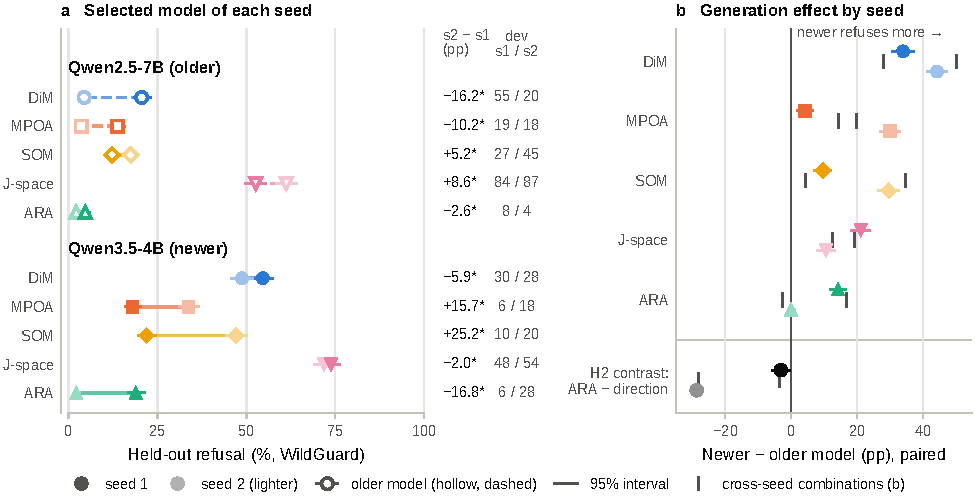
\includegraphics[width=\textwidth]{figures/fig13_seed_heldout.pdf}
\caption{\textbf{Seed sensitivity of held-out, judged refusal on the small pair (Qwen2.5-7B $\to$ Qwen3.5-4B).} Each of the ten model $\times$ method cells was optimised twice with 100 TPE trials that differ only in the seed (in three seed-2 runs also in batch size), and the model selected from each run was evaluated on the held-out set. (a) Share of the 972 harmful held-out prompts whose response WildGuard labels a refusal for the seed-1 model (full method colour) and the seed-2 model (lighter), with Wilson 95\% intervals; hollow markers and dashed lines mark the older model. Columns on the right: seed 2 minus seed 1 (percentage points, paired; * = significant, exact McNemar, Holm over the ten cells) and the dev keyword refusals (of 100) of the two selected trials. (b) Generation effect (newer minus older model, paired, Newcombe 95\% intervals; item-bootstrap interval for the H2 row) with seed 1 (upper) and seed 2 (lower, lighter); the grey ticks are the two cross-seed combinations. The bottom row is the H2 contrast (ARA minus the mean of the direction-based methods). The main-study pairs have one seed only.}
\label{fig:seed-heldout}
\end{figure*}
% caption: paper/figures/captions.md (fig13_seed_heldout)

\paragraph{Capability, divergence and over-refusal.} Mean capability change of
the 42 primary models ranged from $-$4.2 to +0.9~pp
(Figure~\ref{fig:capability}) and teacher-forced divergence from 0.004 to
0.279 nats per token (Figure~\ref{fig:divergence}). Capability change was not
correlated with the selected dev KL (Spearman $\rho=-0.03$ [$-$0.29, +0.24],
56 modified models) but was with teacher-forced divergence ($\rho=-0.48$
[$-$0.66, $-$0.24]). Over-refusal on the 350 benign prompts fell significantly
in 41 of the 42 primary models; the exception was the failed Gemma-4-31B DiM
edit.
% src: results/analysis/final_kl_vs_capability_cells.csv; paper/tables/t3_teacher_forced.csv; final_kl_vs_capability.csv (n = 56);
% src: secondary_overrefusal.csv (41 of 42; gemma-4-31b__dim p_holm 0.250).

\begin{figure*}[!htbp]
\centering
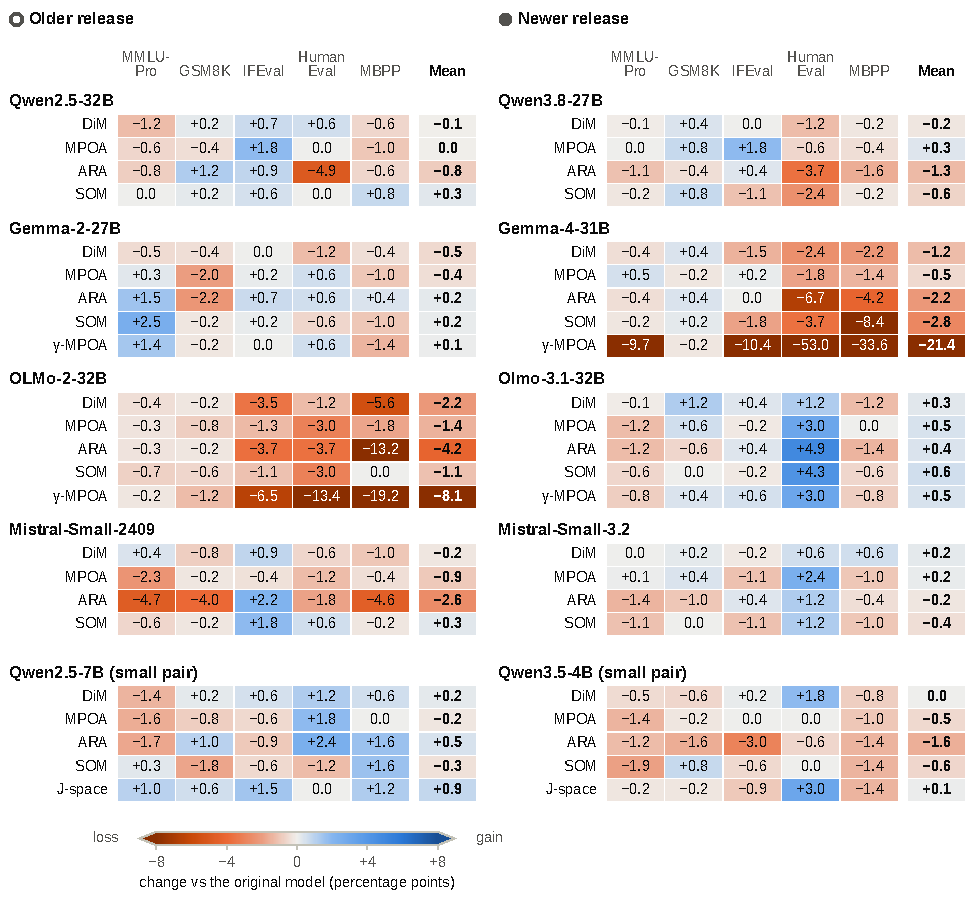
\includegraphics[width=\textwidth]{figures/fig5_capability_deltas.pdf}
\caption{\textbf{Capability change after refusal removal.} Each cell is the benchmark score of the selected model minus that of its own original, in percentage points (pp); the last column is the unweighted mean of the five benchmarks. Orange marks a loss, blue a gain; the scale saturates at $\pm$8 pp and the printed values are exact (beyond the scale: Gemma-4-31B SOM MBPP, $-$8.4 pp; Gemma-4-31B $\gamma$-MPOA MMLU-Pro, $-$9.7 pp; Gemma-4-31B $\gamma$-MPOA IFEval, $-$10.4 pp; Gemma-4-31B $\gamma$-MPOA HumanEval, $-$53.0 pp; Gemma-4-31B $\gamma$-MPOA MBPP, $-$33.6 pp; Gemma-4-31B $\gamma$-MPOA Mean, $-$21.4 pp; OLMo-2-32B ARA MBPP, $-$13.2 pp; OLMo-2-32B $\gamma$-MPOA HumanEval, $-$13.4 pp; OLMo-2-32B $\gamma$-MPOA MBPP, $-$19.2 pp; OLMo-2-32B $\gamma$-MPOA Mean, $-$8.1 pp). Rows align the same method across the older (left) and newer (right) release of a pair; the 8 public community releases are shown in Figure~\ref{fig:community-releases}. One item is worth 0.1--0.61 pp depending on the benchmark and the lm-eval standard error of a single score is 0.7--3.9 pp, so differences of 1--2 pp are within noise (single seed).}
\label{fig:capability}
\end{figure*}
% caption: paper/figures/captions.md (fig5_capability_deltas)

\begin{figure*}[!htbp]
\centering
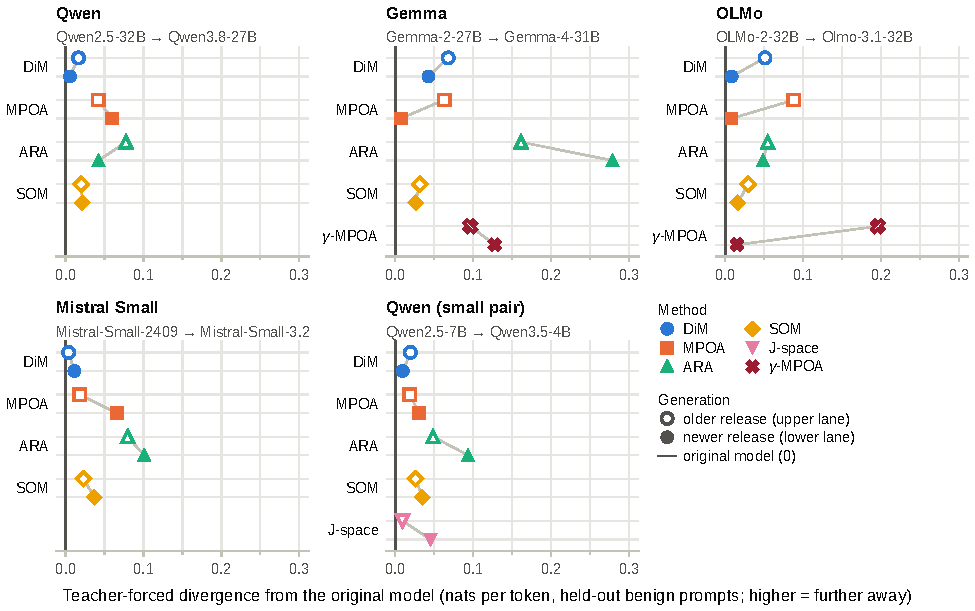
\includegraphics[width=\textwidth]{figures/fig6_divergence.pdf}
\caption{\textbf{Divergence of the refusal-removed models from their originals on benign held-out prompts.} Each dot is the teacher-forced divergence of one selected model: the token-averaged $\log p_{\mathrm{orig}}(y)-\log p_{\mathrm{mod}}(y)$ over the original model's own greedy answers $y$ to the 350 benign held-out prompts; 0 is the original model. Panels are pairs; in each row the older release is in the upper lane (hollow marker) and the newer one in the lower lane (filled), joined by a grey line. The Qwen3.5-4B values also contain an export difference: its evaluated checkpoints lack the 15 mtp.* tensors and store 48 F32 linear-attention tensors (A\_log, norm.weight) as BF16, which by itself changes the log-probabilities. Single seed; no uncertainty intervals are drawn.}
\label{fig:divergence}
\end{figure*}
% caption: paper/figures/captions.md (fig6_divergence)

\paragraph{Development set and search.} On the dev prompts used for search and
selection (Figure~\ref{fig:pareto}), dev keyword counts correlated with
held-out refusal across the 42 primary models ($\rho=0.77$ [0.61, 0.87]), but
the change from older to newer model could differ in sign between the two
sets; for ARA it rose by 20.3 dev refusals on average while the pooled
held-out ARA effect was small (Appendix~\ref{app:moved-results},
Figure~\ref{fig:dev-generation}). The released exports reproduced their
selected trials' dev counts to within two refusals in 37 of 46, and 34 of the
42 core searches reached their selected count by trial 75
(Figure~\ref{fig:search-convergence}).
% src: results/analysis/final_log.txt (d) (rho 0.77 [0.61, 0.87]); paper/figures/captions.md (fig3 "For the text" ARA +20.3);
% src: dev_rescore_groups.csv (37 of 46); final_search_runs.csv (34 of 42 by trial 75).

\begin{figure*}[!htbp]
\centering
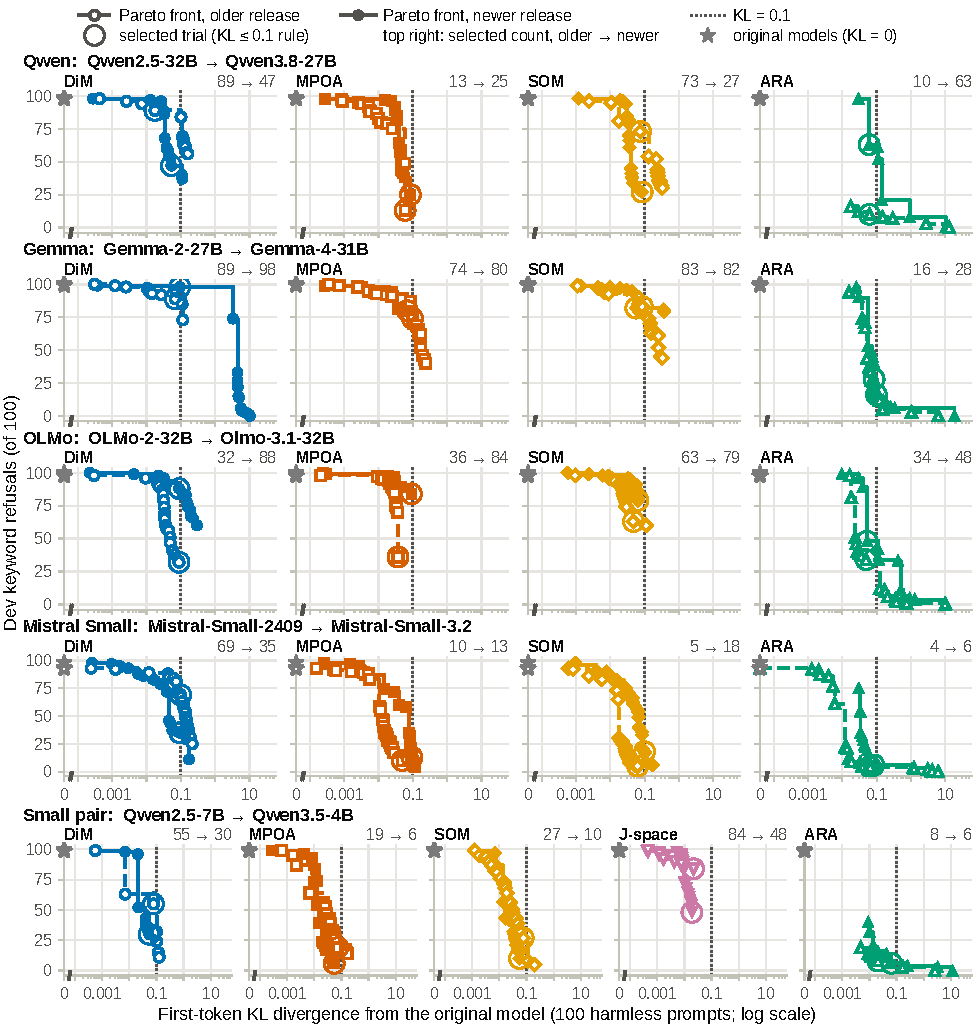
\includegraphics[width=\textwidth]{figures/fig2_pareto_fronts.pdf}
\caption{\textbf{Refusal--KL trade-off explored by each optimisation run (dev set).} Rows are model pairs (older $\to$ newer release), columns refusal-removal methods; J-space was run on the small pair only. Each panel holds two Pareto fronts, one per release (one run each: 100 TPE trials, seed 1): the trials that no other trial of that run beats on both dev keyword refusals and first-token KL divergence; dashed with hollow markers for the older release, solid with filled markers for the newer one. The ring marks the trial chosen by the selection rule (fewest dev keyword refusals at KL $\le$ 0.1); its count is given at the top right of the panel (older $\to$ newer release). Grey stars are the original models (KL = 0). The x axis is logarithmic, with KL = 0 drawn at the left edge behind an axis break; the dotted line is the selection budget KL = 0.1. Every completed trial is shown per run in Figures~\ref{fig:trials-old} and~\ref{fig:trials-new}. Refusal counts are keyword matches on the 100 dev prompts that were also used for optimisation and selection, not held-out refusal rates.}
\label{fig:pareto}
\end{figure*}
% caption: paper/figures/captions.md (fig2_pareto_fronts)

% ------------------------------------------------------------
\subsection{Summary of Key Findings}
\label{sec:res-summary}

Judged by the class-level per-pair effects, H1 was not supported: after
direction-based removal the newer model retained much more refusal in the
OLMo pair, somewhat more in the small, Qwen and Gemma pairs and none in the
Mistral Small pair, and after ARA more in the Qwen and small pairs and less in
the Gemma pair (Table~\ref{tab:pair-effects}). At the point estimate of the
run-to-run standard deviation, the only raw per-pair generation effect that
excluded zero under both variance models was the OLMo direction-based
increase. With run-to-run variance included, the between-pair heterogeneity
of the direction-based effect was high on the percentage-point scale under
the constant variance model ($I^2=80\%$), moderate under the refusal-level
model (46\%) and small on the log-odds scale (20\%). The conjunctive
criterion of H1, more refusal on the newer model for every method, was met by
no main-study pair; it is a secondary and seed-fragile summary, because the
small pair met it with seed~1 but not with seed~2, which erased the ARA
generation effect. H2 held per pair in Gemma and OLMo, but each contrast rests
on one ARA cell; the Gemma contrast lost its interval support under the
refusal-level variance and changed sign with the KL budget on the dev set,
and the Qwen contrast, positive in its point estimate and on the public item
sets (Table~\ref{tab:pair-source}), was indeterminate, because its interval
with run-to-run variance included zero. H3's prediction was not supported:
keyword matching agreed with the judge on average at the tool's window but
disagreed by several points per model.
% 2026-11-08 ARS re-review revision (REV-18, REV-17, NEW-3, NEW-4): H1 verdict led by the class-level per-pair effects;
% conjunctive criterion secondary and seed-fragile (final_seed_generation.csv: small-pair ARA seed1 +14.2, seed2 +0.0 pp,
% p_mcnemar 1); Qwen H2 indeterminate (review_sel_pair_effects.csv qwen H2 pp [-5.9, +53.1]); I2 by variance model
% (revision_heterogeneity.csv 0.798 / 0.458 / 0.201); "at the point estimate" (revision_sigma_pair_verdicts.csv: olmo direction
% raw excl0_level_hi False).
% src: as the subsections above (review_sel_pair_effects.csv; revision_heterogeneity.csv; revision_sigma_pair_verdicts.csv;
% src: revision_kl_budget_effects.csv; review_out_c2_pair_class.csv; review_out_c4_gap_pooled.csv; revision_kw_gap_abs.csv).

% 2026-11-08 adversarial check: the former \clearpage here (flush Results floats) left three figure-only pages
% (Figures 7-9); removed so that Figures 8 and 9 share pages with Discussion text.
